 \documentclass[czech,a4paper,22pt]{article}
 \setlength{\topmargin}{-3.54cm}
 \setlength{\oddsidemargin}{-1cm}
 \setlength{\evensidemargin}{-1cm}
 \setlength{\textwidth}{17.5cm}
 \setlength{\textheight}{25.5cm}

 \usepackage[czech]{babel}
 \usepackage[utf8]{inputenc}
 \usepackage{graphicx}
 \usepackage{subfigure}
 \usepackage{picins}
 \usepackage{amsmath}
 \usepackage{color}
 \usepackage{latexsym}

 \def\modre#1{\textcolor{blue}{#1}}
 \def\algn#1{\mbox{\sc #1}}
 \def\pp{\hglue 2em}
 \def\kw#1{{\bf #1}}
 \begin{document}
{\small
\begin{tabular}{p{.6\textwidth}p{.25\textwidth}}

~

\LARGE{\bf A}

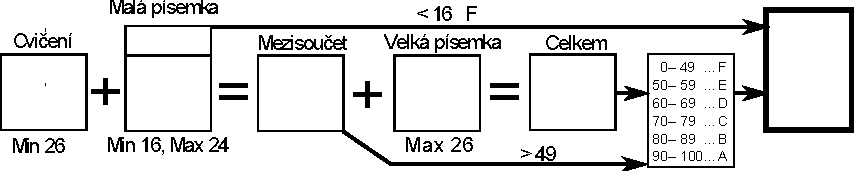
\includegraphics[width=10cm]{hlavicka.pdf}
    &
\begin{tabbing}
  \hspace{1.5cm} \= \hspace{2cm} \= \ 
   Prijmeni: \> 
\rule{3cm}{.1mm}\[.3cm]
   Jmeno:  \> 
\rule{3cm}{.1mm}\[.3cm]
   Cvicici:  
   \> $\Box$ Matyas \> $\Box$ Chludil\[.3cm]
   Skupina: 
   \> $\Box$ ct, 12:45 \> $\Box$ st, 12:45 \ 
   \> $\Box$ ct, 14:30 \> $\Box$ st, 14:30 \ 
   \> $\Box$ ct, 16:15 \> $\Box$ st, 16:15 \ 
   \> $\Box$ ct, 18:00 \> $\Box$ st, 18:00 \ 

\end{tabbing}
\end{tabular}
}
\begin{enumerate}n
	\large{\item jak jsi se dnes vyspal?
 \}
\hrule
\begin{description}
 \item[b] dobre
 \item[c] spatne
 \item[d] velmi spatne
 \item[e] nespal jsem
\end{description}
\hrule
	\large{\item kolik mas deti?
 \}
\hrule
\begin{description}
 \item[b] 0
 \item[c] 1
 \item[d] 2
 \item[e] vice
\end{description}
\hrule
	\large{\item co je dnes za den?
 \}
\hrule
\begin{description}
 \item[b] pondeli
 \item[c] streda
 \item[d] sobota
 \item[e] nevim
\end{description}
\hrule
\end{enumerate}
\newpage
{\small
\begin{tabular}{p{.6\textwidth}p{.25\textwidth}}

~

\LARGE{\bf A}

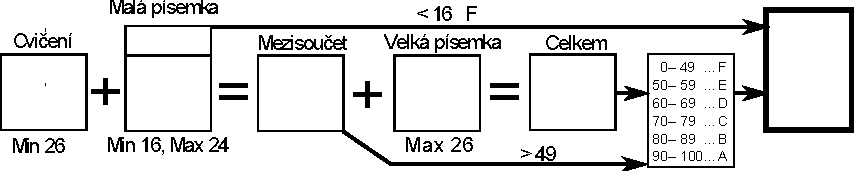
\includegraphics[width=10cm]{hlavicka.pdf}
    &
\begin{tabbing}
  \hspace{1.5cm} \= \hspace{2cm} \= \ 
   Prijmeni: \> 
\rule{3cm}{.1mm}\[.3cm]
   Jmeno:  \> 
\rule{3cm}{.1mm}\[.3cm]
   Cvicici:  
   \> $\Box$ Matyas \> $\Box$ Chludil\[.3cm]
   Skupina: 
   \> $\Box$ ct, 12:45 \> $\Box$ st, 12:45 \ 
   \> $\Box$ ct, 14:30 \> $\Box$ st, 14:30 \ 
   \> $\Box$ ct, 16:15 \> $\Box$ st, 16:15 \ 
   \> $\Box$ ct, 18:00 \> $\Box$ st, 18:00 \ 

\end{tabbing}
\end{tabular}
}
\begin{enumerate}n
	\large{\item v kolik rano vstavas?
 \}
\hrule
\begin{description}
 \item[b] pred patou
 \item[c] mezi patou sestou
 \item[d] mezi sestou sedmou
 \item[e] po sedme
\end{description}
\hrule
	\large{\item jsi retard?
 \}
\hrule
\begin{description}
 \item[b] uplny
 \item[c] myslim ze nekdy ano
 \item[d] asi nejsem, ale jisty to neni
 \item[e] nejsem retard
\end{description}
\hrule
	\large{\item typ tveho mobilu
 \}
\hrule
\begin{description}
 \item[b] dotykovy nejnovejsi
 \item[c] dotykovy stary model
 \item[d] starsi model bez dotykove obrazovky
 \item[e] alternativni zbran
\end{description}
\hrule
\end{enumerate}
\newpage
\end}document}
